\section{Results}
\subsection{Mechanical Results}
After my design iterations, tests and hours of CAD and 3d printing the final result for the mechanical design of the SmallKat is something we were definitely proud of.

  \begin{figure}[H]
                    \centering
                    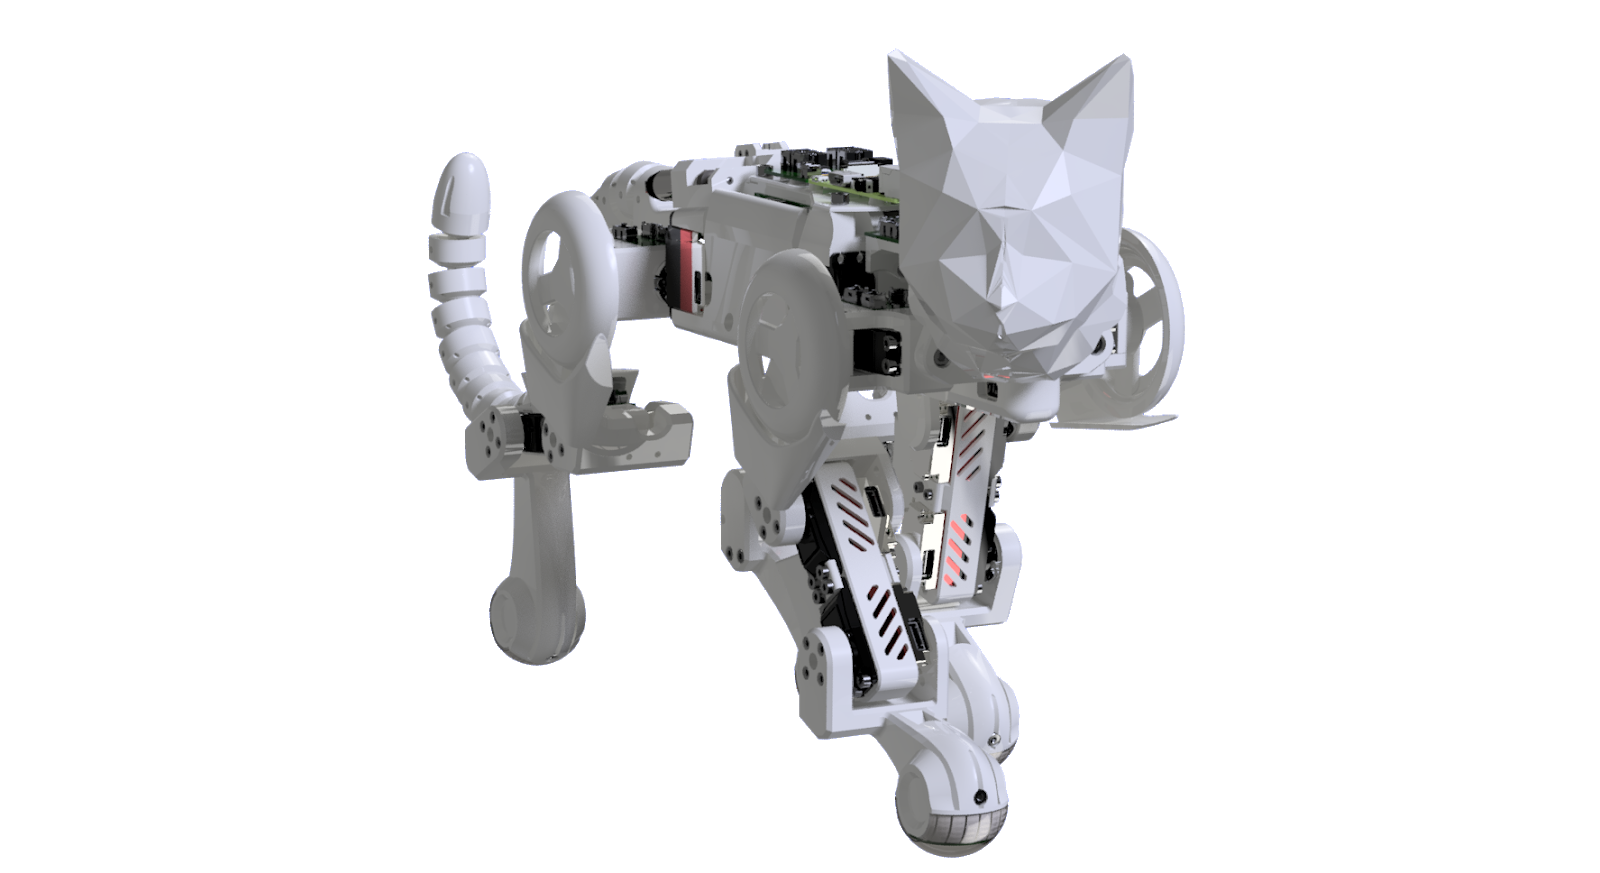
\includegraphics[width=0.7\textwidth]{figures/SmallKatFrontView.png}
                    \caption{CAD rendering of a front view of the cat}
                    \label{SmallKatFrontView}
            \end{figure}  

4 DOF legs were created using custom servo motors. These were 3d printed using readily available hardware to allow for simple construction, deconstruction, modification and adaptability. Each leg had an extensive range of motion to allow for both static and dynamic walking gaits. Aesthetic pieces were added to improve the overall look of the robot as well as provide guards for electrical wires. Each foot was equipped with a molded poly-urethane foot that housed the custom foot sensors. Two different sized legs were made for the front and back of the robot to more closely mimic the actual dimensions and structure of a cat.

A continuum tail was developed to allow for balance control of the cat and add a more realistic look to the robot. After a series of tests with dual extruded designs, the tail was ultimately made using 18 universal joints. This design was split into two individually controlled segments that are each controlled by two Maxon motors and a spring. Each motor has an encoder and is paired with a limit switch that allows the custom tail board to home and control the position of the tail. The kinematics for the tail were tested and implemented to allow for simple control that involved sending two angles to each segment of the tail. 

The rest of the mechanical design involved the creation of a body and head. The final design housed all the custom electronics boards, on board computer, battery and sensors. Everything the robot needs to run is on board allowing for future work to be done completely untethered. The head of the robot was designed with two degrees of freedom allowing it to work with the tail to provide some stability and balance control. The same model was used for this design as was used in previous versions of SmallKat. The only difference being size. The head of this design is big enough to house additional cameras and sensors for future iterations of the project.

A full mass analysis of the robot was done to determine center of masses for each individual link and the system as a whole. By applying densities of our specific materials in CAD we were able to approximate the mass to be around 9.4 pounds. The actual mass of the robot weighed in at around 9.6 pounds. The discrepancy is most likely due to some error in the densities of our PCB boards and 3d printed parts. However the masses were close enough to give us confidence in the position of the center of masses for each component on the robot. This data was put into bowler studios for future work into dynamic walking gaits. The position of the center of mass of the whole robot was also used to place the IMU.



\subsection{Electrical Results}
Custom Servo motor controllers were developed to fit within the existing footprint of the JX-HV5932MG servos that allowed for position, Velocity and torque control along with live tunable PID, coriolis and gravity gains to allow for smooth control and operation. 

A series of pressure sensing foot sensors were developed to allow for triangulation of the force vector being applied to each foot of the robot. This will allow during future development to determine when and where contact has been made during a step cycle in a gait.

A 9DOF IMU board was developed to use the communication protocol of the rest of the robot. By utilizing the BNO055 IMU, a number of data sets are able to be collected, the standard sets of gyroscope, magnetometer and accelerometer in X, Y \& Z along with the gravity vector with respect to the IC and the Euler angles roll, pitch \& heading. This data will allow for the dynamics of the system to be obtained quickly and accurately to be used in computing the corrective gait cycles.

An integrated charging board that reports the status of the battery pack to the motherboard and in turn motors (for accurate force calculation) was developed in order to easily charge the battery pack with in the robot at the highest charging current permitted by the specifications of the battery pack and reporting back to the motherboard in order to prevent from over draw of the system, which would result in damage caused to the battery pack. 

The motherboard developed for this robot handles all communication through out the system including communication to and from the motors, IMU, foot sensors and battery charger. The motherboard also handles communication back and forth to the integrated on board computer through USB HID where all the kinematics and gaits are processed using data from both the updated trajectory pose and the information returned from the system. 

\subsection{Software Results}
A successful implementation of a static walking gait was achieved using Bowler Studio, Despite this a great deal of time and effort was put into developing both a static and dynamic walking gait in IHMC using integrated libraries and tools in increase the optimization at time of computation as well as to generate the most optimal step cycle, however this was abandoned before completion due to a lack of time.
\subsection{Overarching Results}
In end an aesthetically pleasing 4DoF quadrupedal platform was successfully designed using a series of custom sensors, motors and accessory boards. This combined with the successful implementation of a static walking gait and improved kinematics to utilize the 4DoF of each leg for an orientation angle allowed us to begin the tuning of the walking gait on the robot. In combinations to the static walking gait developed, a more dynamic gait began development in both Matlab and IHMC using their available tools and libraries for optimization.
\begin{figure}[H]
            \centering
            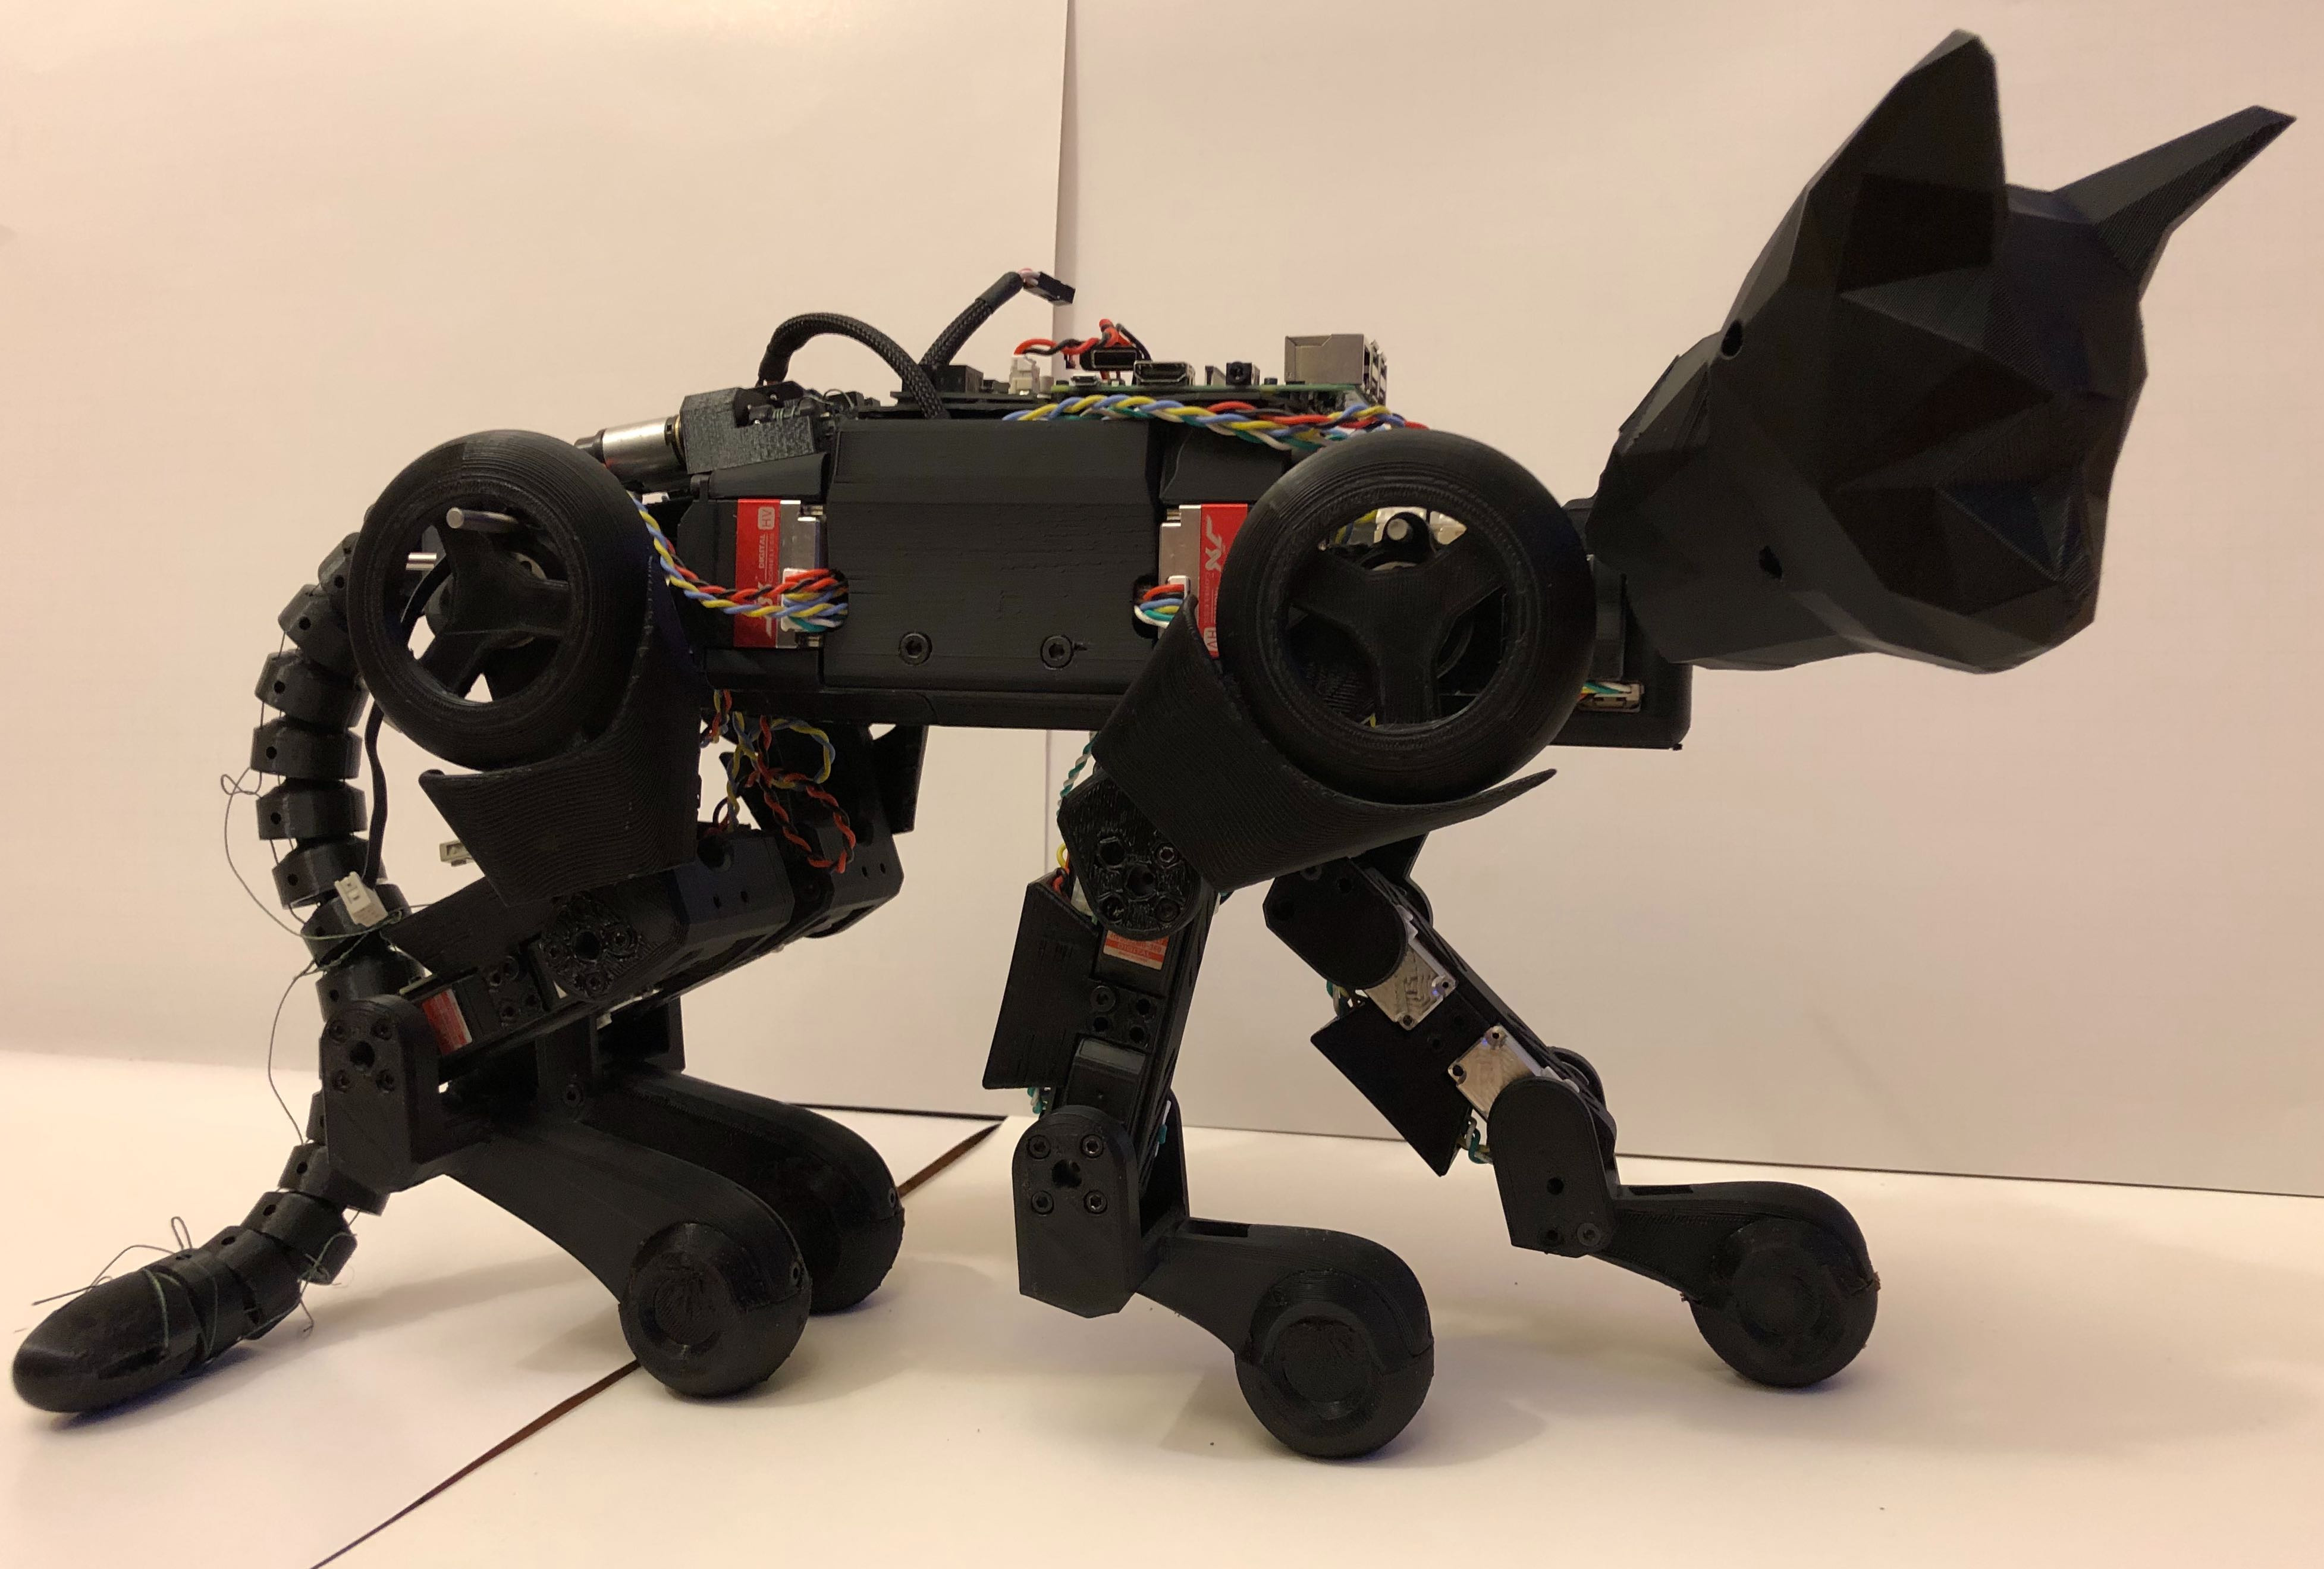
\includegraphics[width=120mm]{figures/FinalRobot.jpg}
            \caption{Final Robot}
            \label{fig:FinalRobot}
\end{figure}

% Add finished robot picture / rendering in this section
